\newpage
ҒТАМР 06.73.07
\hfill {\bfseries \href{https://doi.org/10.58805/kazutb.v.3.24-517}{https://doi.org/10.58805/kazutb.v.3.24-517}}

\sectionwithauthors{Р.Қ. Елшібаев}{БАҒАЛЫ ҚАҒАЗДАР НАРЫҒЫН МЕМЛЕКЕТТІК РЕТТЕУ МӘСЕЛЕЛЕРІ}

\begin{center}
{\bfseries Р.Қ. Елшібаев}

«Нархоз университеті» КЕАҚ, Алматы, Қазақстан
\end{center}

\envelope Корреспондент-автор: rakymzhan.yelshibayev@bk.ru

Елімізде қор биржасының белсенділігі айтарлықтай арта түсті. Әсіресе
жеке инвесторлар сегментінің кеңеюі байқалады. Ол елдегі экономикалық
тұрақтылыққа, инфляция деңейіне, халықтың нақты табысының өсуіне тікелей
байланысты. Сондықтан да елдегі тұрақтылық, халықтың әл-ауқатын арттыру,
экономикалық өсім, ақша-несие жүйесі, бизнес субъектілерінің
белсенділігі басты назарда болуы тиіс. Жеке тұлғалардың бағалы
қағаздарды сатып алуға қызығушылығының артуына пандемия да өзінің
ықпалын тигізді. Жеке инвесторлар банктік депозиттерге баламалы
көздерді, қосымша табыс табу жолдарын қарастыра бастады. Сонымен қатар
брокерлік қызметтерді цифрландыру барлық қызығушылық танытқандарға
инвестициялауға қол жетімділікті қамтамасыз етті.

2020жылдан бастап екінші деңгейлі банктерге брокерлік қызметті жүргізуге
рұқсат берілуі, олардың белсенділігін арттыра түсті. Қазір еліміздің
жекелеген банктері (Халық банк, Банк Центр Кредит) мобильді қосымшалары
арқылы бағалы қағаздарын сатуды іске асыра алады. Қазір тек ірі
компаниялар ғана емес шағын және орта бизнес субъектілерінің де бағалы
қағаздар нарығындағы белсенділігін жоғарылату бойынша жұмыстар жасалып
жатыр. Сондықтан да бағалы қағаздар нарығына бастапқы кезеңде
мемлекеттің араласуы, қолдау және реттеу бойынша жүйелі жұмыстар атқаруы
өте маңызды.

Мақалада елімізде қор нарығын дамытудың қажеттілігі және мемлекеттік
реттеу мәселелері қарастырылған. Бағалы қағаздар нарығын мемлекеттік
реттеудің маңызы, негізгі мақсаты және іске асыру құралдары мен негізгі
тәсілдері көрсетілген, сондай-ақ, өзекті мәселелері анықталып, оларды
шешу жолдары ұсынылған.

{\bfseries Түйін сөздер:} қор нарығы, бағалы қағаздар, эмитент, инвестор,
трейдер, брокер, диллер, мемлекеттік реттеу, Қазақстандық қор биржасы.

\sectionheading{ВОПРОСЫ ГОСУДАРСТВЕННОГО РЕГУЛИРОВАНИЯ РЫНКА ЦЕННЫХ БУМАГ}

\begin{center}
{\bfseries Р.К. Елшибаев}

НАО «Университет Нархоз», Алматы, Казахстан,

e-mail: rakymzhan.yelshibayev@bk.ru
\end{center}

В стране значительно возросла активность фондовой биржи. Особенно
заметно расширение сегмента частных инвесторов. Это напрямую зависит от
экономической стабильности в стране, уровня инфляции, роста реальных
доходов населения. Поэтому в центре внимания должны быть стабильность в
стране, повышение благосостояния населения, экономический рост,
денежно-кредитная система, активность субъектов бизнеса. На рост
интереса физических лиц к покупке ценных бумаг повлияла и пандемия.
Частные инвесторы начали рассматривать альтернативные источники
банковских депозитов, способы получения дополнительных доходов. Кроме
того, цифровизация брокерских услуг обеспечила всем желающим доступ к
инвестированию.

С 2020 года банки второго уровня получили разрешение на ведение
брокерской деятельности, что повысило их активность. Сейчас отдельные
банки страны (Народный банк, Банк Центр Кредит) могут осуществлять
продажу ценных бумаг через мобильные приложения. Сейчас ведется работа
по повышению активности на рынке ценных бумаг не только крупных
компаний, но и субъектов малого и среднего бизнеса. Поэтому очень важно,
чтобы государство на начальном этапе проводило системную работу по
вмешательству, поддержке и регулированию рынка ценных бумаг.

В статье рассматривается необходимость развития фондового рынка и
вопросы государственного регулирования в стране. Указаны важность,
основная цель, инструменты и методы осуществления государственного
регулирования рынка ценных бумаг, а также выявлены актуальные проблемы и
предложены пути их решения.

{\bfseries Ключевые слова:} фондовый рынок, ценные бумаги, эмитент,
инвестор, трейдер, брокер, дилер, государственное регулирование,
Казахстанская фондовая биржа.

\sectionheading{ISSUES OF STATE REGULATION OF THE SECURITIES MARKET}

\begin{center}
{\bfseries R.K. Yelshibayev}

JSC Narxoz University, Almaty, Kazakhstan,

e-mail: rakymzhan.yelshibayev@bk.ru
\end{center}

The activity of the stock exchange has increased significantly in the
country. The expansion of the segment of private investors is especially
noticeable. This directly depends on the economic stability in the
country, the level of inflation, and the growth of real incomes of the
population. Therefore, the focus should be on stability in the country,
improving the well-being of the population, economic growth, the
monetary system, and the activity of business entities. The pandemic
also influenced the growing interest of individuals in buying
securities. Private investors began to consider alternative sources of
bank deposits, ways to generate additional income. In addition, the
digitalization of brokerage services provided everyone with access to
investing.

Since 2020, second-tier banks have received permission to conduct
brokerage activities, which has increased their activity. Now individual
banks of the country (Halyk Bank, Bank Center Credit) can sell
securities through mobile applications. Now work is underway to increase
activity in the securities market not only of large companies, but also
of small and medium-sized businesses. Therefore, it is very important
that the state at the initial stage carries out systematic work to
intervene, support and regulate the securities market.

The article discusses the need to develop the stock market and issues of
government regulation in the country. The importance, main goal, tools
and methods of implementing state regulation of the securities market
are indicated, and current problems are identified and ways to solve
them are proposed.

{\bfseries Key words:} stock market, securities, issuer, investor, trader,
broker, dealer, state regulation, Kazakhstan Stock Exchange.

\begin{multicols}{2}
{\bfseries Кіріспе.} Елімізде бағалы қағаздар нарығын дамыту және реттеу
қаржы секторының тиімділігіне тікелей ықпал етеді. Сондықтан да бұл
мәселе мемлекет басшысының басты назарында. Қор биржасының жеткілікті
деңгейде дамымауы, халықтың қаржылық сауаттылығының төмендігі, бағалы
қағаздармен жұмыс жасауда қажетті білімдер мен дағдылардың болмауы
қарапайым халықтың алаяқтарға алдануына, қаржы пирамидасына сеніп
қалуына алып келеді. Осыған байланысты бұл бағытта
теориялық-әдістемелік, тәжірибелік, ғылыми ізденістердің қажеттілігі мен
маңыздылығы жоғары деп айтуға болады. Еліміз егемендігін алғаннан бастап
қазіргі кезге дейін бағалы қағаздар нарығына қатысты бірқатар
нормативтік-құқықтық актілер әзірленіп, жыл өткен сайын өзгерістер мен
толықтырулар енгізіліп отырды. Соның нәтижесінде бағалы қағаздарды
шығару мен айналымға енгізу бойынша экономикалық қатынастар жүйесінде
жаңа құқықтық орта қалыптастырылды. Алайда бағалы қағаздар нарығын
дамыту мен реттеудің жүйелі тәсілдерінің болмауынан бұл нарық бүгінгі
таңда өзінің инвестициялық функциясын жеткілікті деңгейде орындай алмай
отыр. Қазақстанның бағалы қағаздар нарығын дамыту мен мемлекеттік реттеу
аясындағы іргелі зерттеулердің тапшылығы мәселенің өзектілігін
көрсетеді.

{\bfseries Материалдар және әдістер.} Зерттеу жүргізу барысында
эмпирикалық, субъектілік-объектілік, жүйелік, дедуктивтік және
салыстырмалы талдау әдістері қолданылды. Бұл әдістердің әрқайсысы сәйкес
зерттеу міндеттерін шешу үшін функционалдық мүмкіндіктеріне байланысты
пайдаланылды. Бұл зерттеуде теориялық-эмпирикалық әдістерді қолдану
мемлекеттік реттеу объектісі ретінде Қазақстан Республикасы бағалы
қағаздар нарығының экономикалық мәнін неғұрлым тереңінен түсінуге
мүмкіндік берді.

Бағалы қағаздар нарығын мемлекеттік реттеу жүйесін инфрақұрылымдық
қамтамасыз етуді зерттеу кезінде ақпаратты жинау әдісі және қажетті
материалды тиімді іздеу, топтастыру, өңдеу және қорытындылау үшін
абстрактілеу әдісі ішінара қолданылды.

Нарықтың негізгі экономикалық көрсеткіштерін зерттей отырып автор
жүйелік және салыстырмалы талдау әдістерін қолданды.

Зерттеудің мақсаты -- бағалы қағаздар нарығын мемлекеттік реттеу жүйесін
жетілдіру және дамыту бағыттарын анықтау.

Зерттеу гипотезасы бағалы қағаздар нарығын реттеуді жетілдіру елімізде
қор нарығын дамыту мен тартымдылығын жоғарылатуға мүмкіндік
беретіндігімен сипатталады.

Мақаланың ғылыми жаңашылдығы бағалы қағаздар нарығын мемлекеттік реттеу
қазіргі кезге дейін қалай жүргізілді және алдағы уақытта қандай бағытта
даму қажеттілігін айқындау, нарықтағы өзекті мәселелер және оларды шешу
жолдарын ұсынуда көрініс тапқан.

Зерттеу нәтижелері. Мақаланың негізгі ғылыми нәтижесі бағалы қағаздар
нарығын мемлекеттік реттеудің өзекті мәселелері анықталып, оларды шешу
жолдары ұсынылды.

Бағалы қағаздар нарығы және оның жұмыс жасау механизмінің өзекті
мәселелерін зерттеумен көптеген ғалымдар және практик-мамандар айналысып
келеді. Зерттеу тақырыбы бойынша жарияланған еңбектердің көпшілігінде
елімізде қолайлы инвестициялық ахуалды қалыптастыру арқылы халықтың
әл-ауқатын жақсарту мәселелері қамтылған. Қор нарығын қарқынды дамытуда
және тиімді қызметін қамтамасыз етуде бағалы қағаздар нарығының рөлі,
мемлекеттің ықпал ету дәрежесі, қандай құралдар мен әдіс-тәсілдер арқылы
жоғары нәтижелерге қол жеткізуге болатындығы жеткілікті деңгейде
қарастырылмаған.

{\bfseries Нәтижелер мен талқылау.} Бағалы қағаздар нарығы осындай
қағаздардың эмиссиясы мен айналымы бойынша оның субъектілерінің
арасындағы экономикалық қатынастар жиынтығын білдіреді. Бағалы қағаздар
нарығының субъектілері ретінде эмитенттер, инвесторлар мен нарықтың
кәсіби қатысушыларын айта аламыз {[}1{]}.

Қазақстанда бағалы қағаздар нарығы екі үлкен бөлікке бөлінген:
ұйымдастырылған бағалы қағаздар нарығы және ұйымдастырылмаған бағалы
қағаздар нарығы.

Бағалы қағаздар нарығының қатысушыларын шартты түрде бірнеше топқа
бөлуге болады:

\begin{enumerate}
\def\labelenumi{\arabic{enumi}.}
\item
  Жеке және институционалдық инвесторлар.
\item
  Бағалы қағаздар шығаратын эмитенттер.
\item
  Бағалы қағаздар нарығының кәсіби қатысушылары (бағалы қағаздар
  нарығында қызметін жүзеге асыруға лицензиясы бар ұйымдар).
\item
  Сауданы ұйымдастырушылар (қор биржасы немесе орталық депозитарий)
  {[}2{]}.
\end{enumerate}

Бағалы қағаздар нарығын мемлекеттік реттеу - бұл бағалы қағаздар нарығы
қатысушыларының іс-әрекетін реттеуге бағытталған мемлекеттің
уәкілеттілік берген ұйымының іс-әрекеті.

Мемлекеттік реттеудің негізгі мақсаты -- бағалы қағаздар нарығының одан
әрі дамуы мен тиімді қызмет етуін қолдау. Ол келесілер арқылы қамтамасыз
етіледі:

\begin{itemize}
\item
  нарықтың барлық қатысушыларының жұмысына қолайлы жағдай жасау және
  реттеу;
\item
  нақты сұраныс және ұсыныс негізінде нарықтағы баға белгілеуге бақылау
  жүргізу;
\item
  нарықтағы ойыншылардың тәуекелінің сыйақысы үшін әлеуетті капиталды
  қайта бөлудің тиімді механизмін жасау;
\item
  контрагенттердің әртүрлі сипаттағы әділетсіз әрекеттерінен нарық
  қатсушыларын қорғау; Мәселен, әділетсіз бәсеке, инсайдерлік ақпаратпен
  сату, алаяқтық т.б. сақтау;
\item
  бағалы қағаздар сферасында тиімді салық салу жүйесін қалыптастыру;
\item
  жаңа нарықтарды ұйымдастыру, олардың құрылымдарын, бастамалары мен
  жаңашылдықтарын қолдау;
\item
  бағалы қағаздар нарығын дамыту кезінде қоғамдық мүдделердің бұзылуына
  жол бермеу {[}3{]}.
\end{itemize}

Бағалы қағаздар нарығын мемлекеттік реттеу тәсілдерін келесі сурет
түрінде көрсетуге болады (1-сурет).

Бағалы қағаздар нарығын мемлекеттік реттеу тәсілдері
\end{multicols}

\begin{figure}[H]
	\centering
	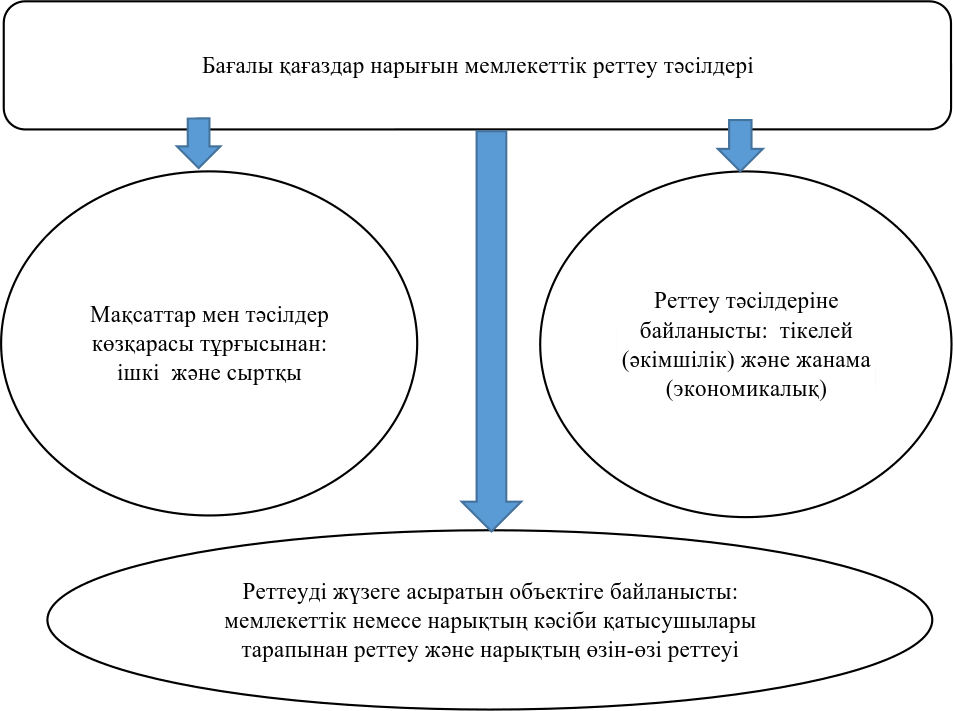
\includegraphics[width=0.7\textwidth]{assets/340.1}
	\caption*{1 - сурет. Бағалы қағаздар нарығын мемлекеттік реттеу тәсілдері Ескерту -- зерттеулер негізінде автормен әзірленген}
\end{figure}

\begin{multicols}{2}
«Бағалы қағаздар нарығы туралы» заңға сәйкес, мемлекеттік реттеу
органдары келесідей міндеттерді шешуі тиіс:

\begin{itemize}
\item
  бағалы қағаздар нарығының кәсіби қатысушыларының, эмитенттердің
  қызметіне қатысты міндетті талаптарды және оның стандарттарын
  белгілеу;
\item
  бағалы эмиссиялық қағаздар шығару мен эмиссиялар проспектісін тіркеу
  және ондағы қарастырылған шарттар мен міндеттемелерді эмитенттердің
  сақтауын бақылау;
\item
  бағалы қағаздар нарығының кәсіби қатысушыларының қызметін лицензиялау;
\item
  меншік иелерінің құқықтарын қорғау жүйесін құру және олардың
  құқықтарын қаржы нарығының кәсіби қатысушыларының және эмитенттердің
  сақтауын бақылау;
\item
  лицензиясыз кәсіпкерлік қызметпен айналысатын тұлғалардың іс-әрекетіне
  тиым салу және шектеу, сондай-ақ, бағалы қағаздар нарығы
  қатысушыларының кәсіби және білім деңгейін жоғарылатуды ұйымдастыру
  {[}4{]}.
\end{itemize}

Жоғарыда айтып өткеніміздей бағалы қағаздар нарығын реттеуді нарық
қатысушыларының өздері іске асыруы мүмкін. Ол үшін нарықтың кәсіби
қатысушылары (брокерлер мен дилерлер) коммерциялық емес ұйымдарға
бірігеді. Мұндай ұйымдардың мақсаты -- бағалы қағаздар нарығын реттеу
процесіне мемлекеттік реттеуші ұйымдармен бірге қатысу. Мұндай жағдайда
мемлекет өздерінің реттеуші функцияларының бір бөлігін береді. Алайда
мұндай ұйымдарды мемлекеттік деп атауға болмайды, оларды өзін-өзі
реттеуші ұйымдар деп атайды {[}5{]}.

Қазақстанда жалғыз толыққанды өзін-өзі реттейтін ұйым -- Қазақстандық
қор биржасы (KASE). Оның жарғысына сәйкес негізгі міндеттеріне мыналар
жатқызылады:

\begin{itemize}
\item
  бағалы қағаздар нарығында кәсіби қызметтің қолайлы шарттарын
  қамтамасыз ету;
\item
  нарықта кәсіби этика стандарттарын қолдау;
\item
  мемлекеттік реттеу органдарында кәсіби қатысушылардың мүдделерін
  қорғау;
\item
  бағалы қағаздармен операциялар жүргізудің ережелері мен стандарттарын
  белгілеу;
\item
  олардың орындалуын бақылау {[}6{]}.
\end{itemize}

KASE индексі қазақстандық бағалы қағаздар нарығының даму динамикасын
сипаттайтын негізгі индикатор болып табылады.

Қазір қазақстандық қор биржасында келесідей қаржы құралдары айналымда
жүр:

\begin{itemize}
\item
  жедел келісім-шарттар: стандартталған жеткізілмеген АҚШ долларындағы
  фьючерс;
\item
  ҚР қаржы министрлігімен берілген мемлекеттік бағалы қағаздар;
\item
  ҚР Ұлттық Банкімен берілген бағалы қағаздар;
\item
  ҚР Қаржы министрлігінің мемлекеттік мүлік және жекешелендіру
  департаментімен сатуға қойылған акциялардың мемлекеттік пакеті;
\item
  Екінші деңгейлі банктердің депозиттік сертификаттары;
\item
  Мемлекеттік емес бағалы қағаздар: облигациялар, жай, атаулы,
  артықшылығы бар акциялар.
\end{itemize}

Мемлекеттік бағалы қағаздардың табыстылығы жоғары емес, бірақ, олар
сенімділіктің жоғары дәрежесін иеленеді. Сондықтан да халықтың бір тобы
тәуекелге бармастан, өздерінің қаражаттарын осындай бағалы қағаздарға
салу дұрыс деп есептейді.

Қазақстандық қор биржасында мемлекеттік бағалы қағаздармен сауда жасау
тәсілі электрондық үздіксіз қарсы аукцион әдісі болып табылады. Ол
қойылған бағамға сәйкес ең жақсы қарсы баға бойынша жасырын контр
әріптеспен автоматты түрде мәміле жасауға негізделген. Сол себепті
абстрактілеу әдісі көзқарасы тұрғысынан мемлекеттік бағалы қағаздар
нарығының динамикасын бақылау едәуір күрделі және тиімсіз болып
көрінеді.

Автордың пікірі бойынша, нарықты реттеу мен дамыту жөнінде мемлекеттік
шаралардың тиімділігін бағалау үшін мемлекеттік емес бағалы қағаздардың
едәуір динамикалық нарығына және оның институционалдық инвесторына назар
аудару қажет. Сонымен қатар бағалы қағаздар нарығының дамуы елімізде
қаржы секторының дамуымен тікелей байланысты екендігін атап өту қажет.

Елімізде қаржы секторын дамытудың негізгі жеті бағыты анықталған. Олар
келесілер:

\begin{itemize}
\item
  қаржылық тұрақтылық және оған деген сенімді қолдау;
\item
  тұрақты дамуға көшу (инновациялар, технологиялар, бизнес-модельдер мен
  құзіреттіліктер);
\item
  қаржылық қызметті тұтынушылардың құқықтары мен мүдделерін қорғау;
\item
  экономиканы қаржыландыру және банктік сектордың дамуы;
\item
  қаржылық мүдделерді қорғау құралы ретінде сақтандыру нарығының дамуы;
\item
  экономиканы қаржыландырудың қосымша каналы ретінде бағалы қағаздар
  нарығын дамыту;
\item
  банктік емес сектор мен микроқаржыландыруды дамыту {[}7{]}.
\end{itemize}

{\bfseries Қорытынды.} Жүргізілген зерттеулер негізінде бағалы қағаздар
нарығын дамыту мен мемлекеттік реттеу жүйесіндегі мынадай өзекті
мәселелер анықталды:

\begin{itemize}
\item
  нарықтың шектеулі өтімділігі;
\item
  нарық субъектілерінің қызметін реттейтін заңдар мен басқа да
  нормативтік құжаттардағы кемшіліктер;
\item
  сапалы қаржылық құралдардың тапшылығы;
\item
  акционерлер өз кәсіпорнын қор нарығына шығарған жағдайда оны жоғалтып
  алудан қорқуы және жариялы IPO дан бас тартуы;
\item
  листингтік компаниялардың ашықтығының жеткілікті деңгейде болмауы;
\item
  инвесторлардың, әсіресе портфельдік және шағын кәсіби емес
  инвесторлардың құқытары мен мүдделерін қорғаудың нақты механизмінің
  болмауы.
\end{itemize}

Отандық бағалы қағаздар нарығын қажетті деңгейде дамыту үшін мемлекеттің
уәкілетті органы келесідей іс-шараларды жүзеге асыруы керек:

\begin{enumerate}
\def\labelenumi{\arabic{enumi}.}
\item
  Отандық қор нарығында айналымда болатын өтімді және сенімді қаржылық
  құралдардың тізімін кеңейту.
\item
  Тәуекелдерді басқару жүйесінің сапасын жоғарылата отырып, заманауи
  IT-технологиялардың көмегімен кәсіби қатысушылардың жұмыс жасау
  әдістерін жетілдіру арқылы қаржылық қызмет көрсету сапасын арттыру.
\item
  Эмитенттер мен олардың лауазымды тұлғаларының облигацияларды шығару
  мен орналастыру талаптарын бұзғаны үшін жауапкершілікті жоғарылату.
\item
  Облигацияларды ұстаушылардың өкілдерінің рөлін көтеру және
  функцияларын кеңейту;
\item
  Қазақстандық қор биржасына эмитенттер мен биржа мүшелеріне мониторинг
  жасау мақсатында қосымша функциялар беру.
\end{enumerate}

Зерттеу тақырыбы бойынша жүргізілген ізденістер, ғылыми және іскерлік
әдебиеттерді талдау мен қорытындылау нәтижесінде келесідей маңызды
міндеттерді шешуге назар аудару қажеттілігі анықталды:

\begin{itemize}
\item
  Бағалы қағаздар нарығының тұрақтылығын арттыру. Яғни, бағалы қағаздар
  нарығындағы тәуекелдердің алдын алу және төмендету бойынша іс-шаралар
  әзірлеу. Бағалы қағаздар нарығындағы инвесторлардың мүдделері мен
  құқықтарын қорғауды қамтамасыз ету.
\item
  Экономикалық интеграция жағдайында бағалы қағаздар нарығының
  тиімділігін жоғарылату. Бағалы қағаздар нарығында сұранысты
  ынталандыру мен көтеру, білікті инвесторлар институтының қызмет ету
  механизмін жетілдіру, брокерлік ұйымдардың функционалы мен
  мүмкіндіктерін кеңейту.
\item
  Инфрақұрылымды жетілдіру және бағалы қағаздар нарығын сапалы дамыту
  үшін оңтайлы жағдай жасау. Эмитенттерге қойылатын листигтік талаптар
  мен қор биржасының ресми тізімінің құрылымын реформалау.
\item
  Бағалы қағаздар нарығының әлеуетін кеңейту, соның ішінде экономиканың
  қажеттіліктеріне жауап беретін қаржылық өнімдер есебінен. Бағалы
  қағаздар нарығында ұсынысты қалыптастыру мен қолдау және эмитенттердің
  акцияларын алғашқы орналастыруға шығару.
\end{itemize}

Зерттеу тақырыбы бойынша белгілі бір шамада ғылыми ізденістердің
жасалғанына қарамастан отандық бағалы қағаздар нарығының дағдарысқа
тұрақтылығын жоғарылату және халықтың қайталама нарықтағы белсенділігін
арттыру мәселесі аз зерттелген күйінде қалып отыр. Дегенмен жүргізілген
зерттеулер мен жасалған ұсыныстар автордың келтірген гипотезасының
дұрыстығын нақтылай түседі.
\end{multicols}

\begin{center}
{\bfseries Әдебиеттер}
\end{center}

\begin{noparindent}
1.
Magill, M., Quinzii M. Normative properties of stock market
equilibrium with moral hazard. Journal of Mathematical Economics.
-2011.-Vol.44(7--8).- P. 785-806.
https://doi.org/10.1016/j.jmateco.2006.09.006

2.
Симинин Ю.Г. Правовое регулирование рынка ценных бумаг.
Учебно-методическое пособие. -- Костанай: КГУ имени А. Байтурсынова,
2012. - 92с.

3.
Teall, J.L. Regulation of Trading and Securities Markets // Financial
Trading and Investing. -2013.-Vol. 147. -Iss. 2. --P. 93-115.
DOI:10.1016/B978-0-12-391880-2.00004-6

4.
Закон Республики Казахстан «О рынке ценных бумаг» от 02.07.2003года №
461 (обновленный с изменениями и дополнениями по состоянию на
19.06.2024г.) URL: https://zakon.uchet.kz/rus/docs/Z03000 0461\_

5.
Cabán-García, M. The impact of securities regulation on the earnings
properties of European cross-listed firms. The International Journal
of Accounting. -2011. -Vol. 44(3). - P.279-304.

https://doi.org/10.1016/j.intacc.2009.06.005

6.
Еркебаев, Р.К. Фондовые рынки и биржевое дело: Учебник. - Алматы:
Принт-С., 2016. -- 395 с. ISBN 978-601-289-048-8

7.
Как будут развивать финансовый сектор в Казахстане до 2030года. //
Курсив 02.07.2022.
URL:
https://kz.kursiv.media/2022-07-02/kak-budut-razvivat-v-kazahstane-finansovyj-sektor-do-2030-goda/
\end{noparindent}

\begin{center}
{\bfseries References}
\end{center}

\begin{noparindent}
1. Magill, M., Quinzii M. Normative properties of stock market
equilibrium with moral hazard. Journal of Mathematical Economics. -2011.
-Vol. 44.(7-8).- P.785-806

https://doi.org/10.1016/j.jmateco.2006.09.006

2. Siminin Ju.G. Pravovoe regulirovanie rynka cennyh bumag.
Uchebno-metodicheskoe posobie. - Kostanaj: KGU imeni A. Bajtursynova,
2012. -- 92s. {[}in Russian{]}

3. Teall, J.L. Regulation of Trading and Securities Markets // Financial
Trading and Investing. -2013.-Vol. 147(2). - P. 93-115.
DOI:10.1016/B978-0-12-391880-2.00004-6

4. Zakon Respubliki Kazahstan «O rynke cennyh bumag» ot 02.07.2003goda №
461 (obnovlennyj s izmenenijami i dopolnenijami po sostojaniju na
19.06.2024g.) URL: https://zakon.uchet.kz/rus/docs/Z03000 0461\_ {[}in
Russian{]}

5. Cabán-García, M. The impact of securities regulation on the earnings
properties of European cross-listed firms. The International Journal of
Accounting. -2011. -Vol. 44(3).- P.279-304.

https://doi.org/10.1016/j.intacc.2009.06.005

6. Erkebaev, R.K. Fondovye rynki i birzhevoe delo: Uchebnik. -- Almaty:
Print-S., 2016.-395 s. ISBN 978-601-289-048-8 {[}in Russian{]}

7. Kak budut razvivat\textquotesingle{} finansovyj sektor v Kazahstane
do 2030goda. // Kursiv 02.07.2022.

URL:
https://kz.kursiv.media/2022-07-02/kak-budut-razvivat-v-kazahstane-finansovyj-sektor-do-2030-goda/
{[}in Russian{]}
\end{noparindent}

\emph{{\bfseries Автор туралы мәліметтер}}

\begin{noparindent}
Елшібаев Р.Қ. -- Экономика ғылымдарының кандидаты, Нархоз
университетінің профессоры, Алматы, Қазақстан, e-mail:
rakymzhan.yelshibayev@bk.ru
\end{noparindent}

\emph{{\bfseries Information about the author}}

\begin{noparindent}
Yelshibayev R.K. -- Сandidat of Economic sciences, Professor of the
University of Narkhoz, Almaty Kazakhstan,e-mail:
rakymzhan.yelshibayev@bk.ru
\end{noparindent}


